%%%%%%%%%%%%%%%%%%%%%%%%%%%%%%%%%%%%%%%%%%%%%%%%%%%%%%%%%%%
%%%%% 													%%%%%
%%%%%	Aller voir le lien suivant :					%%%%%
%%%%%													%%%%%
%%%%%	http://fr.wikibooks.org/wiki/LaTeX				%%%%%
%%%%%													%%%%%
%%%%%%%%%%%%%%%%%%%%%%%%%%%%%%%%%%%%%%%%%%%%%%%%%%%%%%%%%%%

\documentclass[a4paper,12pt]{report}

%%%%%%%%%%%%%%%%%%%%%%%%%%%%%%%%%%%%%%%%%%%%%%%%%%%%%%%%%%%
%%%%% 	pour le français et les accents 	      %%%%%
%%%%%%%%%%%%%%%%%%%%%%%%%%%%%%%%%%%%%%%%%%%%%%%%%%%%%%%%%%%

\usepackage[utf8]{inputenc} 
\usepackage[french]{babel} 

%%%%% 		Pour les marges de la page			 %%%%%%%%
\usepackage[top=2cm, bottom=2cm, left=2cm, right=2cm]{geometry}
%%%%%%%%%%%%%%%%%%%%%%%%%%%%%%%%%%%%%%%%%%%%%%%%%%%%%%%%%%%


\usepackage[T1]{fontenc}

%%%%% Pour les url %%%%%
\usepackage{hyperref}

%%%%% Gestion des numeros de sous-sous-sections %%%%%
\usepackage{titlesec}
\setcounter{secnumdepth}{3}

%%%%% Gestion des sous sous section dans la TOC %%%%%
\setcounter{tocdepth}{3}

%%%%% Insertion des images %%%%%
\usepackage{graphicx}

%%%%% Gestion du centrage des titres %%%%%
\usepackage{sectsty}
\usepackage{lipsum}

%%%%% Demarrage à 0 des sections %%%%%%
\renewcommand{\thesection}{\arabic{section}}
\setcounter{section}{0}


%%% Maketitle metadata
\newcommand{\horrule}[1]{\rule{\linewidth}{#1}} 	%ligne horizontale

\parindent=1cm

%%% Forcer les images à rester dans leur section
\usepackage[section]{placeins}

%%% Utiliser un formatage pour le code 
\usepackage{listings}
\usepackage{color}
\definecolor{lightgray}{rgb}{.9,.9,.9}
\definecolor{darkgray}{rgb}{.4,.4,.4}
\definecolor{purple}{rgb}{0.65, 0.12, 0.82}

\lstdefinelanguage{JavaScript}{
  keywords={typeof, new, true, false, catch, function, return, null, catch, switch, var, if, in, while, do, else, case, break},
  keywordstyle=\color{blue}\bfseries,
  ndkeywords={class, export, boolean, throw, implements, import, this},
  ndkeywordstyle=\color{darkgray}\bfseries,
  identifierstyle=\color{black},
  sensitive=false,
  comment=[l]{//},
  morecomment=[s]{/*}{*/},
  commentstyle=\color{purple}\ttfamily,
  stringstyle=\color{red}\ttfamily,
  morestring=[b]',
  morestring=[b]"
}

\lstset{
   language=JavaScript,
   backgroundcolor=\color{lightgray},
   extendedchars=true,
   basicstyle=\footnotesize\ttfamily,
   showstringspaces=false,
   showspaces=false,
   numbers=left,
   numberstyle=\footnotesize,
   numbersep=9pt,
   tabsize=2,
   breaklines=true,
   showtabs=false,
   captionpos=b
}


%%%%%%%%%%%%%%%%%%%  PAGE DE GARDE %%%%%%%%%%%%%%%%%%%%%%
\title{	
		\horrule{0.5pt} \\[0.5cm]
		\huge(73) PJI Architecture TOR sur\\ navigateur web \\
		\horrule{0.5pt} \\[0.5cm]
}
\author{
		\normalfont 								\normalsize
        Franquenouille Kevin\\[-3pt]		\normalsize
       	Cornette Damien\\[-3pt]		\normalsize
       	Git Repository : \url{https://github.com/kfranquenouille/PJI-TOR.git} \\[-3pt]		\normalsize
       	\\
       	\normalfont
       	Suivi par : Julien Iguchi-Cartigny\\[-3pt]		\normalsize
}
\date{
		\normalfont 								\normalsize
        Année universitaire : 2014-2015\\[-3pt]		\normalsize
}

%%%%%%%%%%%%%%%%%%%  DEBUT DU RAPPORT %%%%%%%%%%%%%%%%%%%%
\begin{document}

\maketitle	

%%%%%%%%%%%%%%%%%%%  DEBUT INTRODUCTION %%%%%%%%%%%%%%%%%%%%
\newpage
\begin{center}
\section*{Introduction}
\end{center}
\paragraph{}
Tor est un projet pour le support de l'anonymat en dissimulant les communications entre un client web et un serveur. Le mécanisme s'appuie sur un ensemble de relais de confiance disposés sur des serveurs. 
\paragraph{} 
Le nombre limité de relais (moins de 5000) et la confiance dans leur non-compromission peut être considéré comme une limitation de l'approche de Tor. Un moyen d'outrepasser cette limitation serait de limiter le rôle du serveur a un simple relais et de laisser les clients gérer l'anonymat dans le système. 
\paragraph{}
Afin de rendre le système le plus pratique et adoptable pour multiplier les chemins possibles, une idée serait de ne s'appuyer que sur des technologies webs (http, javascript) pour que chaque navigateur puisse devenir un client.
\paragraph{}
Le but de ce projet est d'étudier la faisabilité de l'approche à l'aide de technologie comme websocket. Le cas d'étude sera limité à un simple chat (saisie limitée à 140 caractères).

%%%%%%%%%%%%%%%%%%%  FIN INTRODUCTION %%%%%%%%%%%%%%%%%%%%

%%%%%%%%%%%%%%%%%%%  DEBUT TABLE DES MATIERES %%%%%%%%%%%%%%%%%%%%
\tableofcontents
%%%%%%%%%%%%%%%%%%%  FIN TABLE DES MATIERES %%%%%%%%%%%%%%%%%%%%

%%%%%%%%%%%%%%%%%%%  DEBUT %%%%%%%%%%%%%%%%%%%%
\newpage
\section{Description générale du projet}
	\subsection{Problématique}
	\paragraph*{}
	Le but de ce projet était de mettre en place une "simulation" du réseau TOR via un navigateur web. Pour cela, nous avons pu voir avec Julien Iguchi-Cartigni les technologies que l'on pouvait utiliser. De ce fait, on a pu découpé le projet en 2 parties : 
	\begin{itemize}
		\item[•] Web Cryptography API
		\item[•] WebSocket API
	\end{itemize}
	\paragraph*{}
	Pour réaliser cela, nous devions réaliser cela avec un seul relais client pour débuter puis ensuite le faire avec 3 afin de bien vérifier l'encryptage des messages et que les messages sont bien redirigés vers le prochain relais. De plus, il fallait gérer le système de clés publiques et privées afin que le message ne puisse pas être décodé par n'importe quel utilisateur lambda.
	\begin{figure}[h] %%%%% h = here, t = top, b = bottom
		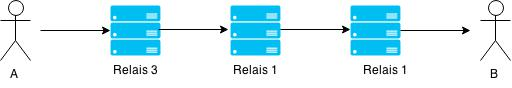
\includegraphics[scale=0.8]{project.jpg}
		\caption{Transfert d'un message de A vers B en passant par 3 relais}
		\label{project}
	\end{figure}
	
	\subsection{Web Cryptography API}
	\paragraph*{}
	Afin de bien crypter les messages envoyés et d'utiliser une technologies assez fiable et récente, nous avons privilégié cette API. En effet, elle est compatible sur presque tous les navigateurs (inclus de base). En revanche, il nous a fallu trouver un bon algorithme de chiffrement.\\
	Dans un premier temps, nous avons utilisé le chiffrement AES-CBC afin de tester et découvrir Webcrypto API et réaliser un premier jet de ce que nous voulions faire. Une fois le messages encrypté 4 fois. Voici un exemple du cryptage :
	\newpage	
	\begin{figure}[h] %%%%% h = here, t = top, b = bottom
		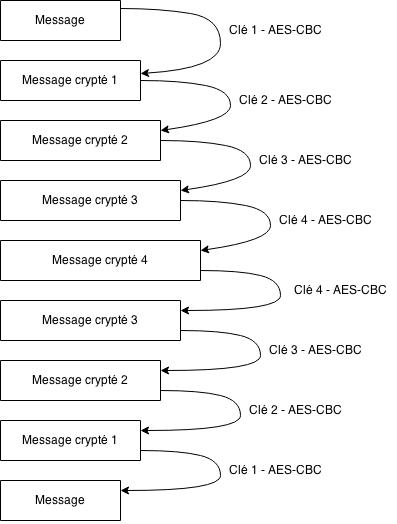
\includegraphics[scale=0.70]{AES.jpg}
		\caption{Cryptage d'un message 4 fois de suite en AES-CBC}
		\label{AES}
	\end{figure}
	\paragraph*{}
	Pour la solution optimale, il est plus préférable d'utiliser un système de clés publiques et de clés privées. Avec l'algorithme RSA-OAEP, celà est possible. Chaque clé générée (l'objet KeyPromise) contient une clé publique et une clé privée. De ce fait, cette solution est plus attendu car elle ressemble très fortement à l'architecture du réseau TOR. Bien entendu, le client doit connaître le chemin afin qu'il puisse créer son message crypté avec les clés publiques des relais correspondants.
	\paragraph*{}
	Ce qu'il faut comprendre en utilisant WebCrypto API, c'est le fait que pour générer une clé, encrypter ou décrypter, nous jouons avec des \textit{Promises}. En Javascript, des \textit{Promises} ou "promesses" en français, sont utilisées pour réaliser des actions asynchrones. En effet, elles représentent des intermédiaires vers des valeurs qui ne sont nécessairement connues lors de leurs créations. Cela permet de gérer des actions asynchrones et de leur associer des gestionnaires d'erreurs. 
	\paragraph*{}
	La principale difficulté qui réside dans le fait d'utiliser des \textit{Promises} est de bien gérer les erreurs mais savoir exactement où le code à échouer. Le fait d'encrypter un message avec une clé publique puis d'encrypter le résultat avec une autre clé publique nécessite obligatoirement une imbrication du code.
	Voici un exemple :
	\begin{lstlisting}
window.crypto.subtle.generateKey({name: "aes-cbc", length: 128}, true, ["encrypt", "decrypt"]).then(function (key) {
  var data = asciiToUint8Array("ceci est un test");
  console.log("Data:");
  console.log("value: ceci est un test")
  console.log(data);
  var algorithm = key.algorithm;
  algorithm.iv = window.crypto.getRandomValues(new Uint8Array(16));

  window.crypto.subtle.encrypt(algorithm, key, data).then(function (ct) {
    console.log("AES-CBC encrypt 1:");
    console.log(new Uint8Array(ct));

    window.crypto.subtle.decrypt(algorithm, key, ct).then(function (pt) {
      console.log("AES-CBC decrypt 1:");
      console.log(new Uint8Array(pt));
      console.log(uint8ArrayToAscii(new Uint8Array(pt)));
    }, handle_error);
  }, handle_error);
}, handle_error);
	\end{lstlisting}
	\paragraph*{}
	Une autre difficulté réside dans le fait de trouver un bon algorithme qui respecte ce que l'on souhaite faire. Par exemple, pour découvrir WebCrypto API, nous avions testé avec la cryptographie AES-CBC comme dans l'exemple précédent.
	Dans ce cas, on constate que l'on a bien une clé qui est générée. En revanche, elle ne respecte par ce que l'architecture TOR exige. La clé n'est pas publique ni privée mais permet juste d'encrypter un message et de le décrypter. Nous avons regardé les différents cryptages disponibles et compatibles et nous avons trouvé RSA-OAEP. Ce dernier gère les clés publiques et privées et permet d'encrypter et de décrypter. D'autres cryptographies RSA possèdent juste les fonctions de signature et de vérification de la signature. Egalement, la cryptographie RSAES-PKCS1-v1\_5	 aurait pu être exploitée mais cette dernière n'est plus disponible dans les navigateurs. C'est donc pour cela que nous avons choisi RSA-OAEP.\\
	Voici un exemple basique avec RSA-OAEP :
	\begin{lstlisting}
window.crypto.subtle.generateKey({name: "RSA-OAEP", modulusLength: 2048, publicExponent: new Uint8Array([0x01, 0x00, 0x01]), hash: {name: "SHA-256"}}, true, ["encrypt", "decrypt"]).then(function (key) {
  var data = asciiToUint8Array("ceci est un test");
  console.log("Data:");
  console.log(uint8ArrayToAscii(data));
  console.log("Public Key");
  console.log(key.publicKey);
  console.log("Private Key");
  console.log(key.privateKey);

  window.crypto.subtle.encrypt({name: "RSA-OAEP"}, key.publicKey, data).then(function (encrypted) {
    console.log(uint8ArrayToAscii(new Uint8Array(encrypted)));

    window.crypto.subtle.decrypt({name: "RSA-OAEP"}, key.privateKey, encrypted).then(function (decrypted) {
      console.log(uint8ArrayToAscii(new Uint8Array(decrypted)));
    }, handle_error);
  }, handle_error);
}, handle_error);
	\end{lstlisting}
	\paragraph*{}
	Egalement, nous avons pu regarder quels sont les algorithmes supportés par la plupart des navigateurs. Nous en avons donc dressé le tableau suivant : 
	\begin{center}
	\begin{tabular}[h]{|*{2}{c|}}
  		\hline
  		Algorithme & Supporté\\
  		\hline
  		RSASSA-PKCS1-v1\_5 & Oui\\
  		\hline
  		RSAES-PKCS1-v1\_5 & Non\\
  		\hline
  		RSA-PSS & Oui\\
  		\hline
  		RSA-OAEP & Oui\\
  		\hline
  		AES-CTR & Oui\\
  		\hline
  		AES-CBC & Oui\\
  		\hline
  		AES-CMAC & Non\\
  		\hline
  		AES-GCM & Oui\\
  		\hline
  		AES-CFB & Oui\\
  		\hline
  		AES-KW & Oui\\
  		\hline
  		SHA-1 & Oui\\
  		\hline
  		SHA-256 & Oui\\
  		\hline
  		SHA-384 & Oui\\
  		\hline
  		SHA-512 & Oui\\
  		\hline
	\end{tabular}
	\end{center}
	Les algorithmes SHA sont des \textit{digest}. Cela sert principalement à créer des table de hachage crypter un message ou une clé par exemple. Dans le code précédent, on peut remarquer que la fonction de hachage mise en place est bien le SHA-256.
	\paragraph*{}
	Une fois que nous avions trouvé l'algorithme et trouver son fonctionnement, nous avons du mettre en place une maquette. Voici donc une image représentative de ce que l'on a testé :
	\begin{figure}[h] %%%%% h = here, t = top, b = bottom
		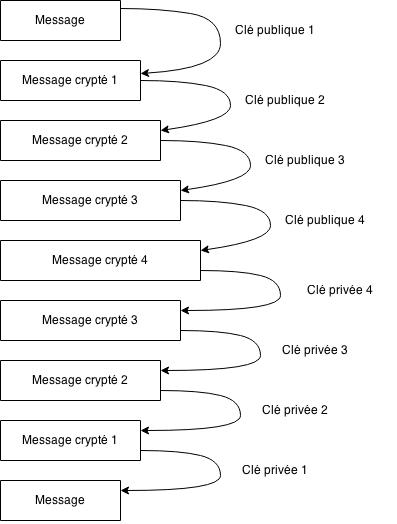
\includegraphics[scale=0.70]{RSA.jpg}
		\caption{Cryptage d'un message 4 fois de suite en RSA-OAEP}
		\label{RSA}
	\end{figure}
	\\
	Dans cet exemple, il faut crypter obligatoirement avec la clé publique et décrypter avec la clé privée correspondante. En effet, les clés publiques sont accessibles à tout le monde alors que les clés privées sont uniquement restreintes au point relais correspondant.

	
	\subsection{WebSocket API}

	\subsection{Architecture de l'application}

\newpage	
\section{Mode d'emploi}
	\subsection{Installer un relais}
	
	\subsection{Configurer un relais}
	
	\subsection{Configurer un client}

	\subsection{Lancer l'application}
	
\newpage	
\section{Tests}
	\subsection{Docker}
	
	\subsection{Cryptographie}
	\paragraph*{}
	Pour la cryptographie avec WebCrypto API, il fallait tester des cas de base. Tout d'abord pour découvrir le fonctionnement, nous avons pris l'algorithme AES-CBC. Puis nous avons généré une clé et encrypté un message de test. Une fois ce message encrypté, nous avons affiché le résultat sous la forme d'une cha\^ine de caractères. Ensuite, pour vérifier que l'on puisse bien décrypter cela, nous l'avons décrypter avec la clé et vérifié que le message décrypté correspondait bien à celui de départ.\\
	Voici le code qui a permis de réaliser cela :
	\begin{lstlisting}
window.crypto.subtle.generateKey({name: "aes-cbc", length: 128}, true, ["encrypt", "decrypt"]).then(function (key) {
  var data = asciiToUint8Array("ceci est un test");
  console.log("Data:");
  console.log("value: ceci est un test")
  console.log(data);
  var algorithm = key.algorithm;
  algorithm.iv = window.crypto.getRandomValues(new Uint8Array(16));

  window.crypto.subtle.encrypt(algorithm, key, data).then(function (ct) {
    console.log("AES-CBC encrypt 1:");
    console.log(new Uint8Array(ct));

    window.crypto.subtle.decrypt(algorithm, key, ct).then(function (pt) {
      console.log("AES-CBC decrypt 1:");
      console.log(new Uint8Array(pt));
      console.log(uint8ArrayToAscii(new Uint8Array(pt)));
    }, handle_error);
  }, handle_error);
}, handle_error);
	\end{lstlisting}
	Une fois ceci réalisé, nous nous sommes posés la question de ce qu'il en est si nous cryptons 4 fois de suite un message. Pour cela, il nous a fallu adapter notre code de manière basique et de tester ce que cela donnait.\\
	Voici l'encha\^inement du code : 
	\begin{lstlisting}
function startCrypto(input_content){
  window.crypto.subtle.generateKey({name: "aes-cbc", length: 128}, true, ["encrypt", "decrypt"]).then(function (key1) {
    var data = asciiToUint8Array(input_content);
    var algorithm = key1.algorithm;
    algorithm.iv = window.crypto.getRandomValues(new Uint8Array(16));

    window.crypto.subtle.generateKey({name: "aes-cbc", length: 128}, true, ["encrypt", "decrypt"]).then(function (key2) {
      var algorithm = key2.algorithm;
      algorithm.iv = window.crypto.getRandomValues(new Uint8Array(16));

      window.crypto.subtle.generateKey({name: "aes-cbc", length: 128}, true, ["encrypt", "decrypt"]).then(function (key3) {
        var algorithm = key3.algorithm;
        algorithm.iv = window.crypto.getRandomValues(new Uint8Array(16));

        window.crypto.subtle.generateKey({name: "aes-cbc", length: 128}, true, ["encrypt", "decrypt"]).then(function (key4) {
          var algorithm = key4.algorithm;
          algorithm.iv = window.crypto.getRandomValues(new Uint8Array(16));

          window.crypto.subtle.encrypt(algorithm, key1, data).then(function (ct1) {
            console.log("AES-CBC encrypt 1:");
            console.log(uint8ArrayToAscii(new Uint8Array(ct1)));

            window.crypto.subtle.encrypt(algorithm, key2, new Uint8Array(ct1)).then(function (ct2) {
              console.log("AES-CBC encrypt 2:");
              console.log(uint8ArrayToAscii(new Uint8Array(ct2)));

              window.crypto.subtle.encrypt(algorithm, key3, new Uint8Array(ct2)).then(function (ct3) {
                console.log("AES-CBC encrypt 3:");
                console.log(uint8ArrayToAscii(new Uint8Array(ct3)));

                window.crypto.subtle.encrypt(algorithm, key4, new Uint8Array(ct3)).then(function (ct4) {
                  console.log("AES-CBC encrypt 4:");
                  console.log(uint8ArrayToAscii(new Uint8Array(ct4)));

                  window.crypto.subtle.decrypt(algorithm, key4, ct4).then(function (pt4) {
                    console.log("AES-CBC decrypt 4:");
                    console.log(uint8ArrayToAscii(new Uint8Array(pt4)));

                    window.crypto.subtle.decrypt(algorithm, key3, pt4).then(function (pt3) {
                      console.log("AES-CBC decrypt 3:");
                      console.log(uint8ArrayToAscii(new Uint8Array(pt3)));

                      window.crypto.subtle.decrypt(algorithm, key2, pt3).then(function (pt2) {
                        console.log("AES-CBC decrypt 2:");
                        console.log(uint8ArrayToAscii(new Uint8Array(pt2)));

                        window.crypto.subtle.decrypt(algorithm, key1, pt2).then(function (pt) {
                          console.log("AES-CBC decrypt 1:");
                          console.log(uint8ArrayToAscii(new Uint8Array(pt)));
                        }, handle_error);
                      }, handle_error);
                    }, handle_error);
                  }, handle_error);
                }, handle_error);
              }, handle_error);
            }, handle_error);
          }, handle_error);
        }, handle_error);
      }, handle_error);
    }, handle_error);
  }, handle_error);
}
	\end{lstlisting} 
	Comme on peut le constater le code devient de plus en plus en illisible si on l'imbrique. Cependant, étant juste le test de découverte, cela avait peut d'importance mais il s'agissait juste de la manière de procéder qui nous intéressait. De ce fait, nous avons appliqué ceci avec la bon cryptage qui est RSA-OAEP. pour le cas d'un seul encryptage, il s'agit a peu de chose près le même cas que AES-CBC. En revanche, pour un encryptage multiple, cela dépend de la taille des données. En effet, nous avons voulu faire varier le \textit{modulusLength}. Cela nous a permis d'avoir un message crypté plus ou moins grand.\\ L'exemple suivant nous a permis de réaliser cela : 
	\begin{lstlisting}
function generateKeys(){
  window.crypto.subtle.generateKey({name: "RSA-OAEP", modulusLength: 512, publicExponent: new Uint8Array([0x01, 0x00, 0x01]), hash: {name: "SHA-1"}}, true, ["encrypt", "decrypt"]).then(function (key) {
    keyGenerate1 = key;
    console.log(keyGenerate1);
    window.crypto.subtle.generateKey({name: "RSA-OAEP", modulusLength: 1024, publicExponent: new Uint8Array([0x01, 0x00, 0x01]), hash: {name: "SHA-1"}}, true, ["encrypt", "decrypt"]).then(function (key2) {
      keyGenerate2 = key2;
      console.log(key2);
      window.crypto.subtle.generateKey({name: "RSA-OAEP", modulusLength: 2048, publicExponent: new Uint8Array([0x01, 0x00, 0x01]), hash: {name: "SHA-1"}}, true, ["encrypt", "decrypt"]).then(function (key3) {
        keyGenerate3 = key3;
        console.log(key3);
        window.crypto.subtle.generateKey({name: "RSA-OAEP", modulusLength: 4096, publicExponent: new Uint8Array([0x01, 0x00, 0x01]), hash: {name: "SHA-1"}}, true, ["encrypt", "decrypt"]).then(function (key4) {
          keyGenerate4 = key4;
          console.log(key4);
          alert("Cles generees");
        }, handle_error);
      }, handle_error);
    }, handle_error);
  }, handle_error);
}	
	\end{lstlisting}
	Une fois les clés générées, il ne nous restait plus qu'à les stocker afin de pouvoir les réutiliser par la suite. De plus, nous avons factoriser le code de l'encryptage et du décryptage afin d'éviter l'imbrication vu comme précédemment. 
		\begin{lstlisting}
function encryptData(key, data, jquerySelector){
  var temp;
  compteur += 1;
  window.crypto.subtle.encrypt({name: "RSA-OAEP"}, key.publicKey, data).then(function (ct1) {
    console.log("RSA-OAEP encrypt "+compteur+" :");
    temp = new Uint8Array(ct1);
    encryptedMsg = new Uint8Array(ct1);
    $( jquerySelector ).text($( jquerySelector ).text()+uint8ArrayToAscii(temp));
    console.log(uint8ArrayToAscii(temp));
  }, handle_error);
  return temp;
}

function decryptData(key, data, jquerySelector){
  window.crypto.subtle.decrypt({name: "RSA-OAEP"}, key.privateKey, data).then(function (pt) {
    console.log("RSA-OAEP decrypt "+compteur+" :");
    encryptedMsg = new Uint8Array(pt);
    $( jquerySelector ).text($( jquerySelector ).text()+uint8ArrayToAscii(encryptedMsg));
    console.log(uint8ArrayToAscii(encryptedMsg));
    compteur -= 1;
    return pt;
  }, handle_error);
}	
	\end{lstlisting}
	L'utilisation de \textit{console.log()} nous a été très utile afin de debugger notre code mais aussi servir de trace pour voir l'utilisation de ce dernier. Une fois ceci fait, l'enchaînement des cryptages et décryptages se fait séquentiellement.\\
	Un exemple est disponible dans la partie ./Webcrypto part/ en affichant la page index.html.
	\subsection{WebSocket}

\newpage	
\begin{center}
\section*{Conclusion}
\end{center}
\end{document}